
\documentclass{article}
\usepackage[utf8]{inputenc}
\usepackage[T5]{fontenc}
\usepackage{graphicx}
\usepackage[margin=1.5cm]{geometry}
\title{Lab 8: RGB--HSV Round Trip}
\author{Nguyễn Thanh Hùng -- 2540056}
\date{}
\begin{document}
\maketitle
RGB2HSV scatters interleaved RGB into separate H, S and V arrays, with H in degrees and S,V in $[0,1]$.
HSV2RGB gathers them back into an RGB image. The notebook saves all three arrays, displays the round trip, checks HSV against Matplotlib and reports maximum RGB reconstruction error.

Kernel timing uses \texttt{time.time()} after JIT warm-up and CUDA synchronization,
averaged over three GPU runs. Device allocation and host/device copies are excluded.
CPU measurements are single runs. Speedup is relative to the stated CPU implementation.
Actual measurements appear after running the notebook on Colab; no timings are assumed here.
\IfFileExists{results.tex}{\begin{center}
\resizebox{\linewidth}{!}{
\begin{tabular}{llll}
\hline
rgb2hsv\_ms & hsv2rgb\_ms & hue\_error & max\_rgb\_error \\
\hline
0.189225 & 0.121673 & 7.08528e-08 & 0 \\
\hline
\end{tabular}
}
\end{center}}{}
\IfFileExists{performance.png}{\begin{center}\includegraphics[width=.75\linewidth]{performance.png}\end{center}}{}
\IfFileExists{images.png}{\begin{center}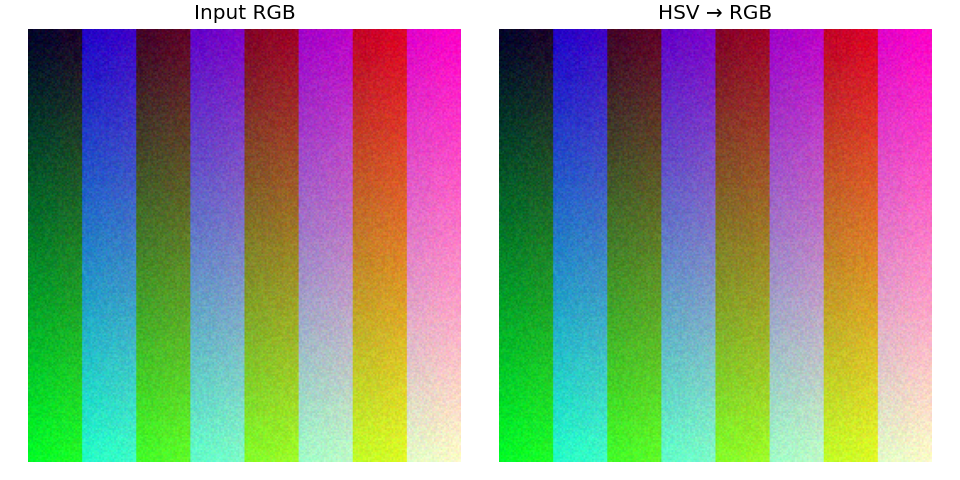
\includegraphics[width=\linewidth]{images.png}\end{center}}{}
\IfFileExists{histograms.png}{\begin{center}\includegraphics[width=.8\linewidth]{histograms.png}\end{center}}{}
\end{document}
